\documentclass[../report.tex]{subfiles}
\begin{document}

    \begin{frame}
        \frametitle{3a: PF Changes in Appearance}
        \begin{figure}[!htb]
            \centering
            \frame{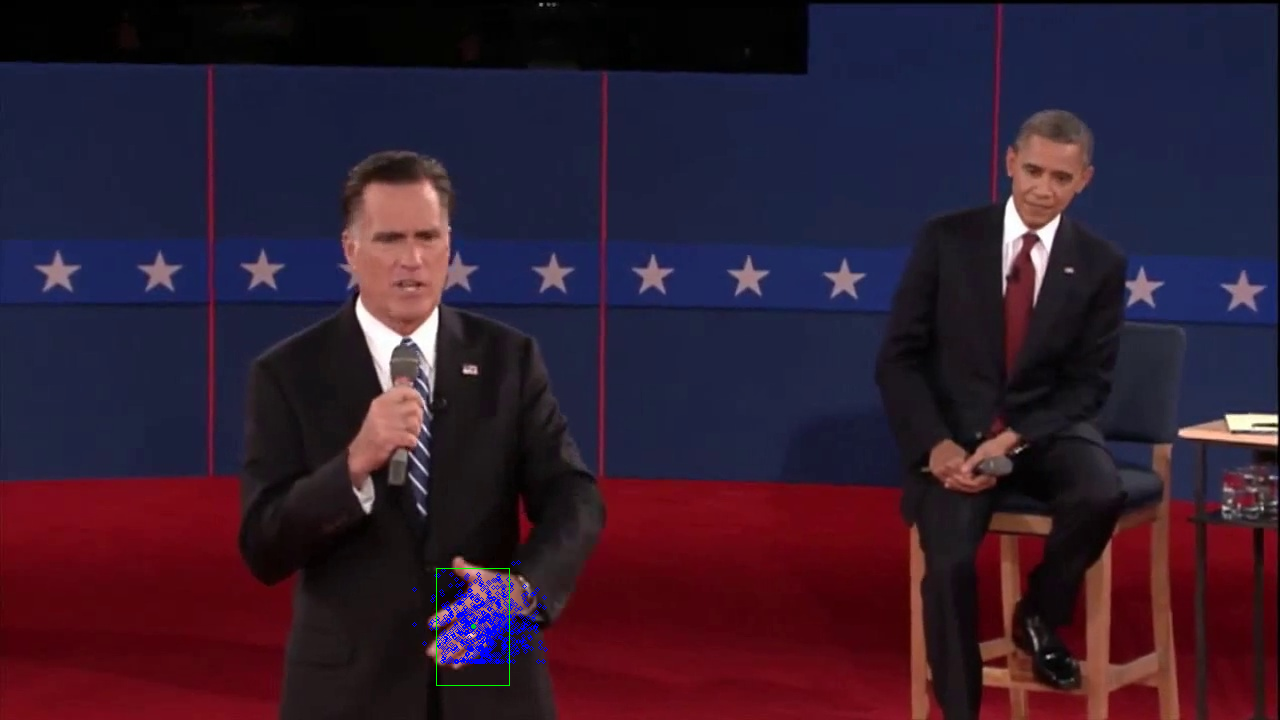
\includegraphics[keepaspectratio,height=0.65\textheight,width=0.45\textwidth]{ps5-3-a-1}}
            \caption{ps5-3-a-1}
        \end{figure}
    \end{frame}

    \begin{frame}
        \frametitle{3a: PF Changes in Appearance (cont)}
        \begin{figure}[!htb]
            \centering
            \frame{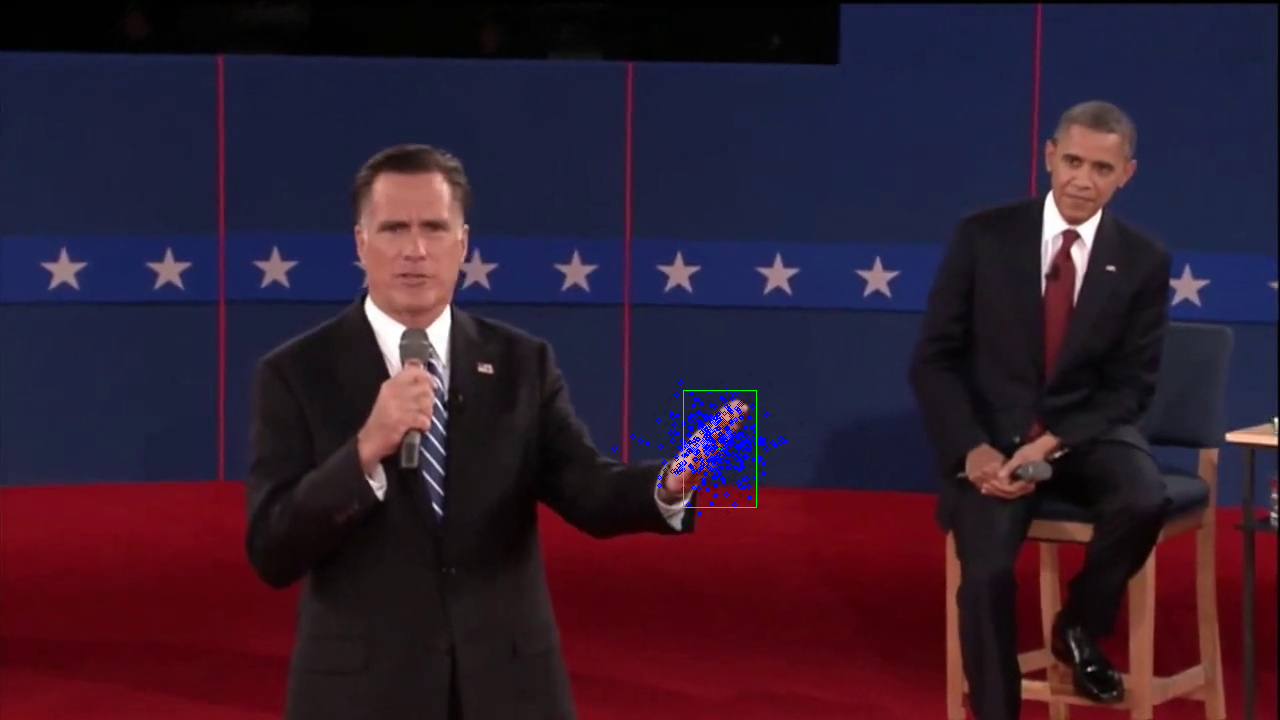
\includegraphics[keepaspectratio,height=0.65\textheight,width=0.45\textwidth]{ps5-3-a-2}}
            \caption{ps5-3-a-2}
        \end{figure}
    \end{frame}

    \begin{frame}
        \frametitle{3a: PF Changes in Appearance (cont)}
        \begin{figure}[!htb]
            \centering
            \frame{
\includegraphics[keepaspectratio,height=0.65\textheight,width=0.45\textwidth]{ps5-3-a-3}}
            \caption{ps5-3-a-3}
        \end{figure}
    \end{frame}
    
\end{document}